%%%%%%%%%%%%%%%%%% PREAMBLE %%%%%%%%%%%%%%%%%%%%%%%%%%%
\documentclass{beamer}
\usepackage{amsfonts,amsmath,oldgerm}
\usepackage{booktabs, caption}
\usepackage[flushleft]{threeparttable}
\usepackage{colortbl}
\usepackage{multirow}
\usetheme{sintef}

\newcommand{\testcolor}[1]{\colorbox{#1}{\textcolor{#1}{test}}~\texttt{#1}}

\usefonttheme[onlymath]{serif}

\titlebackground*{assets/background}

\newcommand{\hrefcol}[2]{\textcolor{cyan}{\href{#1}{#2}}}

\title{Real Estate Inheritance and Wealth Inequality in
Italy}
\subtitle{An Empirical Analysis and Microsimulation of
Tax Policy}
\course{Master's Degree in Economics}
\author{\href{mailto:paoseba01@gmail.com}{Paolo Sebastiani}}
\IDnumber{1954447}
\date{Academic Year 2024/2025}


%%%%%%%%%%%%%%%%%%%%  TITLE  %%%%%%%%%%%%%%%%%%%%%%%%%%
\begin{document}
\maketitle

% This template is released under \hrefcol{https://creativecommons.org/licenses/by-nc/4.0/legalcode}{Creative Commons CC BY 4.0} license

%%%%%%%%%%%%%%%%%%%%  INTRODUCTION  %%%%%%%%%%%%%%%%%%%%%%%%%%
\section{Introduction and Motivation}

\footlinecolor{maincolor}
\begin{frame}{Motivation: Why This Topic?}
    \begin{itemize}
        \item \textbf{Rising Wealth Inequality:} Wealth concentration is a growing concern, and is more pronounced than income inequality in many countries.
        \pause
        \item \textbf{Stagnant Growth:} In a context of economic stagnation, inherited wealth becomes more decisive than labor income for an individual's economic trajectory.
        \pause
        \item \textbf{The Role of Real Estate:} Italy has high home-ownership rates, making real estate the primary component of household wealth and intergenerational transfers.
        \pause
        \item \textbf{Policy Relevance:} Italy's inheritance tax is one of the most lenient in Europe, making an analysis of potential reforms highly relevant.
    \end{itemize}
\end{frame}

\footlinecolor{maincolor}
\begin{frame}{Research Questions}
    \begin{enumerate}
        \item What is the current landscape of \textbf{real estate inheritance and wealth inequality} in Italy?
        \pause
        \item What would be the potential \textbf{redistributive impact} of a revenue-neutral reform of the Italian inheritance tax system?
    \end{enumerate}
\end{frame}


%%%%%%%%%%%%%%%%%%%%  DATA & METHODOLOGY  %%%%%%%%%%%%%%%%%%%%%%%%%%
\section{Data and Methodology}

\footlinecolor{maincolor}
\begin{frame}{Data Source}
    \begin{block}{Bank of Italy's Survey on Household Income and Wealth (SHIW)}
        \begin{itemize}
            \item \textbf{Wave:} 2022.
            \item \textbf{Sample:} 9,641 households, representative of the Italian population.
            \item \textbf{Content:} Detailed information on income, wealth, real and financial assets, and socio-demographic characteristics.
            \item \textbf{Unit of Analysis:} The household, represented by the main income earner.
        \end{itemize}
    \end{block}
\end{frame}

\footlinecolor{maincolor}
\begin{frame}{Methodology}
    \begin{columns}[T]
        \begin{column}{.5\textwidth}
            \textbf{Part 1: Empirical Analysis}
            \begin{itemize}
                \item Descriptive statistics.
                \item Measurement of inequality (Gini, Lorenz Curve).
                \item Analysis of the variables associated with the inheritance status.
            \end{itemize}
        \end{column}
        \pause
        \begin{column}{.5\textwidth}
            \textbf{Part 2: Microsimulation}
            \begin{itemize}
                \item Static non-behavioural model.
                \item Simulates replacing Italy's tax system with 13 international alternatives.
                \item A two-stage "tax-and-transfer" scheme to assess redistributive impact.
            \end{itemize}
        \end{column}
    \end{columns}
\end{frame}

\footlinecolor{maincolor}
\begin{frame}{Limitations of the Study}
    \begin{itemize}
        \item \textbf{Survey Data:} The analysis is based on survey data, which is subject to potential sampling biases and self-reporting errors.
        \pause
        \item \textbf{"Lower-Bound" Analysis:} The analysis is restricted to the inheritance of the household's primary residence, excluding other real estate and financial assets. As a result, the findings represent a "lower-bound" estimate of the total impact of inheritance.
        \pause
        \item \textbf{Static Model:} The microsimulation is static, capturing the immediate "day-after" impact. It does not model potential long-term behavioral changes (e.g., in savings or labor supply).
    \end{itemize}
\end{frame}

%%%%%%%%%%%%%%%%%%%%  EMPIRICAL FINDINGS  %%%%%%%%%%%%%%%%%%%%%%%%%%
\section{Empirical Findings}

\begin{frame}{Finding 1: Wealth Is Far More Unequal Than Income}
    \begin{columns}[T] % The [T] option top-aligns the content in both columns
        \begin{column}{0.7\textwidth}
            \begin{figure}
                \includegraphics[width=0.79\textwidth, keepaspectratio]{Images/lorenz_curves.pdf}
            \end{figure}
        \end{column}
        \begin{column}{0.38\textwidth}
            \vspace{2cm} % Add some vertical space to align text nicely
            \begin{itemize}
                \item \textbf{Gini for Income: 0.365}
                \item \textbf{Gini for Wealth: 0.659}
            \end{itemize} 
        \end{column}
    \end{columns}
\end{frame}


\footlinecolor{maincolor}
\begin{frame}{Finding 2: The "Wealth Floor" Effect}
    \begin{itemize}
        \item Inheritor households (15\% of the population) have \textbf{41\% more total wealth} on average.
        \pause
        \begin{itemize}
            \item This advantage is driven almost entirely by real assets (\textbf{+43\%} relative to the mean).
            \item In contrast, their financial wealth is only marginally higher (\textbf{+3\%}).
        \end{itemize}
        \pause
        \item However, inherited real estate has a counter-intuitive \textbf{equalizing effect} on overall wealth inequality.
        \pause
        \item \textbf{Why?} It acts as a "wealth floor," compressing the lower tail of the wealth distribution. For many beneficiaries, the inherited home is their main asset.
        \pause
        \item The Gini for "self-made" wealth (excluding inherited homes) is \textbf{higher} (0.699) than for total net wealth (0.659).
    \end{itemize}
\end{frame}

\begin{frame}{Finding 2: Visualizing the "Wealth Floor"}
\begin{figure}
        \centering 
        \includegraphics[scale=0.586]{Images/bottom_p_comparison.pdf}
    \end{figure}
\end{frame}


\begin{frame}{Finding 3: The Life-Cycle Effect}

    \begin{columns}[T]
        \begin{column}{0.5\textwidth}
            \begin{figure}
                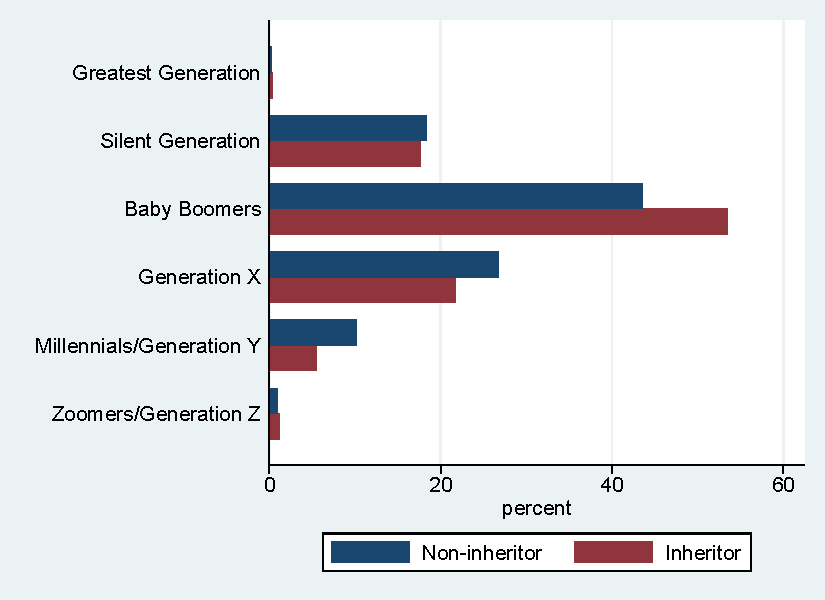
\includegraphics[scale=0.5]{Images/birthcohort_inh.pdf}
            \end{figure}
        \end{column}

        \begin{column}{0.5\textwidth}
            \begin{figure}
                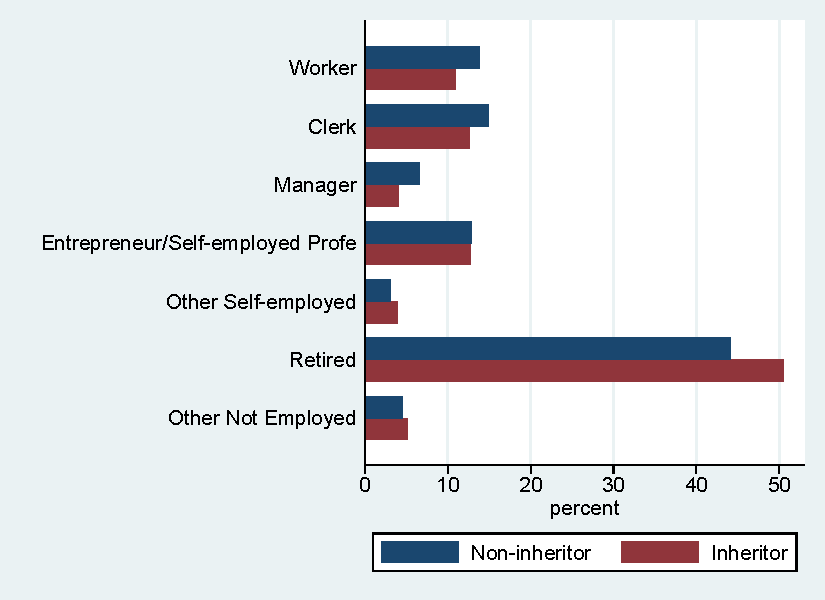
\includegraphics[scale=0.5]{Images/workstatus_inh.pdf}
            \end{figure}
        \end{column}
    \end{columns}

\end{frame}



%%%%%%%%%%%%%%%%%%%%  MICROSIMULATION  %%%%%%%%%%%%%%%%%%%%%%%%%%
\section{Microsimulation of Tax Reform}

\begin{frame}{Microsimulation: The Italian Context}
The current Italian tax system is defined by four main categories, based on the relationship between the deceased and the beneficiary:

\vspace{1em}
\centering\resizebox{\textwidth}{!}{%
\begin{tabular}{l c c}
    \toprule
    \textbf{Beneficiary Relationship} & \textbf{Tax-Free Allowance} & \textbf{Tax Rate} \\
    \midrule
    Spouse \& Direct Relatives &  €1,000,000 & 4\% (on value exceeding allowance) \\
    Siblings & €100,000 & 6\% (on value exceeding allowance) \\
    Other Relatives (up to 4th degree) & None & 6\% (on total value) \\
    All Other Individuals & None & 8\% (on total value) \\
    \bottomrule
\end{tabular}}
\end{frame}


\begin{frame}{Motivation \& Simulation Design}
    \begin{itemize}
        \item Due to the high threshold and low rate, the current tax is \textbf{functionally dormant}. 
        \item My simulation shows that only \textbf{0.8\%} of parent-child inheritances generate any tax revenue.
        \item \textbf{Goal:} To quantify how alternative regimes could make the allocation of housing wealth more equitable.
    \end{itemize}
    \pause
    \begin{block}{Simulation Design: A Two-Stage Process}
    \textbf{Tax Simulation:} "Borrow" the inheritance tax regimes from 13 other countries and apply them to the Italian data to calculate potential revenue. \\
    \textbf{Budget-Neutral Redistribution:} The entire revenue pool is redistributed via four scenarios: \textbf{Targeted} (to the bottom 10\% of households) and \textbf{Universal}. Both are simulated as a \textit{flat lump-sum} and as a \textit{per-capita} transfer.
    \end{block}
\end{frame}

\begin{frame}{Simulation Results: Impact on Wealth Inequality}
\begin{table}[htbp]
\centering
\begin{threeparttable}
\caption{Effects of Different Regimes on the Gini Index}
\label{tab:inequality_effects}
\begin{tabular}{lrrrrr}
\toprule
& & \multicolumn{2}{c}{Lump-Sum} & \multicolumn{2}{c}{Proportional} \\
\cmidrule(lr){3-4} \cmidrule(lr){5-6}
Regime & Tax Effect & to $W_{10}$ & Universal & to $W_{10}$ & Universal \\
\midrule
French   & -0.18 & -2.58 & -1.21 & -2.63 & -1.15 \\
Irish    & -0.35 & -1.26 & -0.53 & -1.25 & -0.50 \\
Japanese & -0.24 & -1.21 & -0.55 & -1.20 & -0.52 \\
Spanish  & +0.04 & \cellcolor{yellow}\textbf{-3.74} & -1.81 & -3.57 & -1.72 \\
\bottomrule
\end{tabular}
\begin{tablenotes}
  \small
  \item Note: All values represent the percentage change ($\Delta$\%) in the Gini index.
\end{tablenotes}
\end{threeparttable}
\end{table}

\end{frame}

\begin{frame}{Political Economy: Who Wins and Who Loses?}
    \begin{figure}
    \includegraphics[scale=0.588]{Images/winners_losers.pdf}
    \end{figure}
\end{frame}

\footlinecolor{maincolor}
\begin{frame}{Simulation Results: Key Findings}
    \begin{enumerate}
        \item \textbf{The Tax-Free Allowance is Crucial:} The allowance, not the top tax rate, is the single most important determinant of a system's redistributive power.
        \pause
        \item \textbf{Redistribution is Key:} The power of the reform comes from \textbf{how the revenue is used}. The direct act of taxing has a negligible effect on inequality.
        \pause
        \item \textbf{Targeted Transfers are Most Effective:} A lump-sum transfer targeted to the poorest decile has the largest impact on reducing the Gini coefficient.
        \pause
        \item \textbf{Universal Transfers are More Feasible:} They create a broad base of support by generating far more 'winners' than 'losers' from the reform.
    \end{enumerate}

\end{frame}


%%%%%%%%%%%%%%%%%%%%  CONCLUSION  %%%%%%%%%%%%%%%%%%%%%%%%%%
\section{Conclusion}

\footlinecolor{maincolor}
\begin{frame}{Summary of Main Findings}
    \begin{itemize}
        \item Wealth inequality in Italy is extremely high, and inherited real estate provides a significant advantage and a "wealth floor" for beneficiaries.
        \pause
        \item Italy's current inheritance tax system is functionally dormant as a redistributive tool.
        \pause
        \item A well-designed, revenue-neutral reform could be a powerful tool to mitigate wealth inequality. The design of the allowance and the use of revenues are the most critical policy choices.
    \end{itemize}
\end{frame}

\footlinecolor{maincolor}
\begin{frame}{Policy Implications \& Future Research}
    \begin{block}{Policy Implications}
        \begin{itemize}
            \item Substantially lowering the €1 million allowance is necessary for any meaningful reform.
            \item Policymakers must decide between statistically efficient targeted transfers and potentially more viable universal transfers.
            \item Administrative challenges (e.g., wealth reporting) must be addressed.
        \end{itemize}
    \end{block}
    \pause
    \begin{block}{Future Research}
        \begin{itemize}
            \item Develop behavioral microsimulation models to account for tax avoidance.
            \item Incorporate all forms of inherited wealth, not just real estate.
            \item Analyze the long-run, multi-generational impacts of reforms.
        \end{itemize}
    \end{block}
\end{frame}


%%%%%%%%%%%%%%%%%%%%  LAST SLIDE  %%%%%%%%%%%%%%%%%%%%%%%%%%
\backmatter

\end{document}
